\documentclass[a4paper,12pt]{article}

%%%%%%%%%%%% PREÁMBULO %%%%%%%%%%%%%%%%%%%%%

% Paquetes

\usepackage[utf8]{inputenc}
\usepackage[spanish,es-tabla]{babel}
\usepackage[T1]{fontenc}

\usepackage{listings}
\usepackage{graphicx}
% Comandos

\renewcommand{\lstlistingname}{Código}
\renewcommand{\lstlistlistingname}{Índice de fragmentos de código fuente}

% Opciones

\title{COMBINATORIA}
\author{Isaac Edgar Camacho}
\date{5 de septiembre de 2018}

%%%%%%%%%%%%%%%%%%%%%%%%%%%%%%%%%%%%%%%%%%%%%%
%margenes

\oddsidemargin=-1cm
\textwidth=18cm
\topmargin=2cm
\textheight=20cm
\evensidemargin -6mm
\oddsidemargin -0.4cm
\textwidth 16.7cm
\textheight 24cm
\topmargin -0.65cm

\begin{document}
\maketitle

\begin{abstract}
Solo sé que no se nada y, \\al saber que no sé nada, \\algo sé; porque sé que no sé nada.
\\y eso me distingue de aquellos que creen saber y no saben nada.
\\Socrates.

\end{abstract}


\section{APRENDIENDO A CONTAR}

\begin{itemize}
\item \textbf{Regla de la suma}\\   
Supongamos que podemos ir de un lugar X a otro Y, ademas supongamos que podemos ir caminando o bien en taxy o en colectivo \\¿De cuantas formas puedo llegar de X a Y? \\ la respuesta por la relga de la suma es de 3 maneras diferentes!!
\begin{center}
\textbf{
Si una primer tarea puede realizarse de \textit{m} formas, mientras que otra tarea puede realizarse de \textit{n} formas, entonces si no se pueden hacer ambas a la vez, cualquiera de ellas pueden realizarse de \textit{m + n} formas.}

\[
\sum_{i=1}^{n}m_{i}
\]
En gral si tenemos n tareas y cada una se puede hacer de m maneras y ninguna se puede hacer simultaneamente
\end{center}

\item \textbf{Regla del producto}\\  
Supongamos que podemos ir de un lugar X a otro Y por ultimo a Z, ademas supongamos que podemos ir de X a Y caminando o en taxy o en colectivo, pero ademas desde Y hasta Z podemos ir en tren o a caballo\\¿De cuantas formas puedo llegar de X a Z? \\ la respuesta por la regla del producto es de 3 x 2 = 6 maneras diferentes!!
\begin{center}
\textbf{
Si un proceso se puede descomponer en dos etapas y el primero tiene \textit{m} resultados posibles, mientras que el segundo tiene \textit{n} resultados posibles, entonces el procedimiento total puede realizarse de \textit{m x n} formas.}

\[
\prod_{i=1}^{n}m_{i}=m_{1}\cdot m_{2}\cdot m_{3} \cdots m_i 
\]
Los procesos son consecutivos es decir que se hacen uno a continuacion de otro.
\end{center}

\section{APLICACIONES}
Siguiendo con las aplicaciones de la regla del producto, ahora contamos disposiciones lineales y una manera sencilla de recordar su clasificaci\'on es usar un cuadro con una serie de preguntas como el que sigue.

\begin {center}
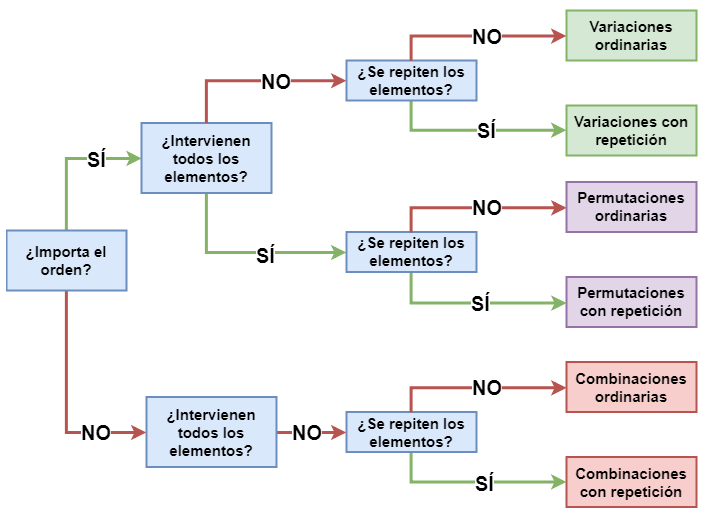
\includegraphics[scale=.3]{combinaciones-17.png}
\end{center}

\item \textbf{Permutaciones sin repeticion de elementos}\\  
Supongamos que tenemos n objetos diferentes, y queremos todas las disposiciones.
\begin{center}
\textbf{
sean objetos $a_1, a_2, a_3, \cdots , a_n$ todas las maneras de disponerlos es decir formarlos uno atras de otros es
\\ $n! = 1 \cdot 2 \cdot 3 \cdots n $}
\end{center}




\item \textbf{Permutaciones con repeticion de elementos}\\  
Ahora los objetos se repiten, es decir que los objetos se pueden agrupar.
\begin{center}
\textbf{
sean n objetos y tenemos $n_1$ de un primer tipo y $n_2$ de un segundo tipo y un ultimo grupo $n_r$ de tipo r ademas los objetos de un mismo tipo son indistinguibles, entonces todas las posibles disposiciones lineales de los n objetos dados se nota:
\begin{equation}
P_{(n,n_1 n_2\cdots n_r)} = \frac{n!}{n_1! \cdot n_2! \cdot n_3! \cdots n_r!}
\end{equation}
}
\end{center}
\end{itemize}

\end{document}